\documentclass[12pt]{article}

\usepackage{amsmath, mathtools}
\usepackage{amsfonts}
\usepackage{amssymb}
\usepackage{graphicx}
\usepackage{colortbl}
\usepackage{xr}
\usepackage{hyperref}
\usepackage{longtable}
\usepackage{xfrac}
\usepackage{tabularx}
\usepackage{float}
\usepackage{booktabs}
\usepackage{caption}
\usepackage{pdflscape}
\usepackage{afterpage}

\usepackage[round]{natbib}

\hypersetup{
    bookmarks=true,         % show bookmarks bar?
    colorlinks=true,       % false: boxed links; true: colored links
    linkcolor=red,          % color of internal links (change box color with linkbordercolor)
    citecolor=green,        % color of links to bibliography
    filecolor=magenta,      % color of file links
    urlcolor=cyan           % color of external links
}

%% Comments

\usepackage{color}

\newif\ifcomments\commentstrue %displays comments
%\newif\ifcomments\commentsfalse %so that comments do not display

\ifcomments
\newcommand{\authornote}[3]{\textcolor{#1}{[#3 ---#2]}}
\newcommand{\todo}[1]{\textcolor{red}{[TODO: #1]}}
\else
\newcommand{\authornote}[3]{}
\newcommand{\todo}[1]{}
\fi

\newcommand{\wss}[1]{\authornote{blue}{SS}{#1}} 
\newcommand{\plt}[1]{\authornote{magenta}{TPLT}{#1}} %For explanation of the template
\newcommand{\an}[1]{\authornote{cyan}{Author}{#1}}

%% Common Parts

\newcommand{\progname}{Mechtronics Enigeering} % PUT YOUR PROGRAM NAME HERE
\newcommand{\authname}{Team 32, Wingman
\\ Edward He
\\ Erping Zhang
\\ Guangwei Tang
\\ Peng Cui
\\ Peihua Jin } % AUTHOR NAMES                  

\usepackage{hyperref}
    \hypersetup{colorlinks=true, linkcolor=blue, citecolor=blue, filecolor=blue,
                urlcolor=blue, unicode=false}
    \urlstyle{same}
                                


\title{Software Requirements Specification\\\progname}

\author{\authname}

\date{}

\begin{document}

\maketitle

\newpage
\pagenumbering{roman}

\tableofcontents

\newpage

\begin{table}[hp]
\caption{Revision History} \label{TblRevisionHistory}
\begin{tabularx}{\textwidth}{llX}
\toprule
\textbf{Date} & \textbf{Developer(s)} & \textbf{Change}\\
\midrule
2022-10-04 & Edward He, Erping Zhang & Revision 0\\
& Guangwei Tang, Peng Cui & \\
& Peihua Jin & \\
\bottomrule
\end{tabularx}
\end{table}

\newpage

\listoftables
\listoffigures

\newpage

\pagenumbering{arabic}

This document describes the requirements for \progname. The template for the Software
Requirements Specification (SRS) is a subset of the Volere
template~\cite{RobertsonAndRobertson2012}. If you make further modifications
to the template, you should explicitly state what modifications were made.

\begin{table}

\end{table}

\section{Project Drivers}

\subsection{The Purpose of the Project}

\subsection{The Stakeholders}

\subsubsection{The Client}

\subsubsection{The Customers}

\subsubsection{Other Stakeholders}

\subsection{Mandated Constraints}

\subsection{Naming Conventions and Terminology}

\subsection{Relevant Facts and Assumptions}

User characteristics should go under assumptions.


\subsection{The Scope of the Work and the Product}

\subsubsection{The Context of the Work}

\subsubsection{Work Partitioning}

\subsubsection{Individual Product Use Cases}

\section{Behavior Description}
\subsection{Assumptions and Dependencies}
\textbf{AD1:} The user can perform simple computer opertions.\\
\textbf{Rationale:} The user can type, moving mousse and clicking on thhe window.\\\\
\textbf{AD2:} The user can understand English.\\\\
\textbf{AD3:} The operation of the project should take place indoors with adequate lighting.\\\\
\textbf{AD4:} All objects can be seen by the product without hiding.\\\\
\textbf{AD5:} Every motion of the user can be seen by the device. 

\subsection{Finite State Machine Description}
To make the behaviour of the product to achieve the target task, the Finite State Machine is created to describe th ebehaviour with detailed description provided after thhe picture. 
\begin{figure}[H]
    \centering
    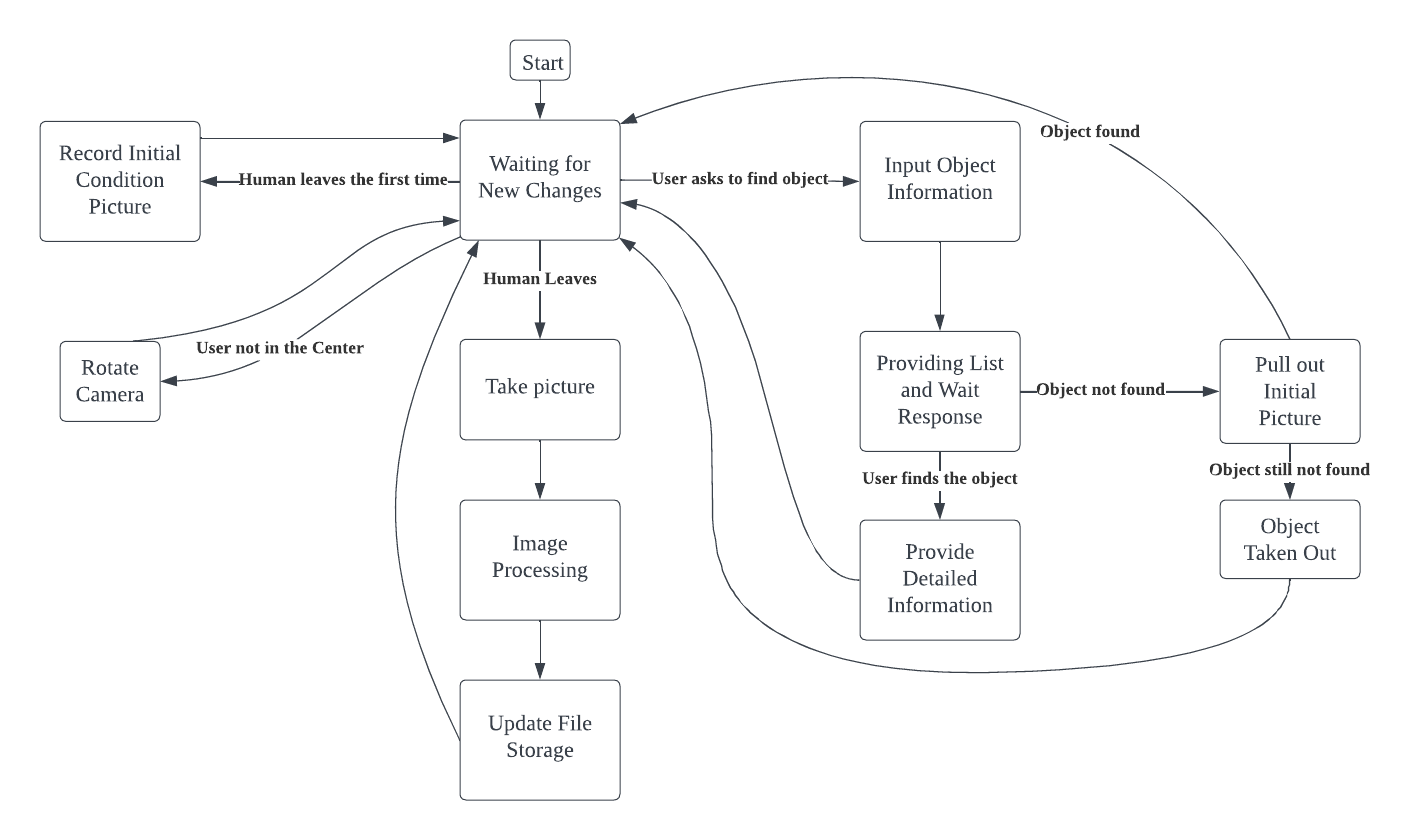
\includegraphics[scale=0.7]{FSM.png}
    \caption{The Picture of Finite  State Machine}
\end{figure}
\textbf{Record Initial Condition:} The device will take a picture of the room as the initial position information for each object and save it to the database. \\\\
\textbf{Waiting for New Changes:} The device will wait for future operations made by human or changes of objects detected by the camera. \\\\
\textbf{Detect Object Movement:} When the device detects the movement of an object that is made by another object (for example, colliding with another object and fall), it will trace the new location oof the object. \\\\
\textbf{Detect Hand Movement:} When the device detects the movement of the user, it will track the movement of the hand to identify which object is being moved and remember its final location. \\\\
\textbf{Updating:} The device will record the updated information (including time, Location, picture of object, and so on) of the object into the database.\\\\
\textbf{Input Object Information} When the user want to find one object in the room, the user interface will ask the user to input information of the object (like size, color, last time saw it, and so on).\\\\
\textbf{Providing List and Wait Response:} After the user has input the information, the system will provide a list of objects with pictures that satisfy the input information.\\\\
\textbf{Provide Detailed Information:} WHen the user find the target object, the device will display the detailed information about the object like showing the current location on the screen. \\\\
\textbf{Pull Out Initial Picture:} When the object is not found in the list, the devide will display the picture taken just after the program starts to let the user find the object.\\\\
\textbf{Object Taken Out:} If the object is still not found, the system will think that thhe object is taken out of the room or is hidden behind another object. \\\\
\textbf{Rotate Camera:} If the device found the human body detected is not in thhe center of the screen or the camera is covered by something else, it will send signals to the motor to rotate the camera until problem sloved. 

\subsection{Use Case Diagram}
\begin{figure}[H]
    \centering
    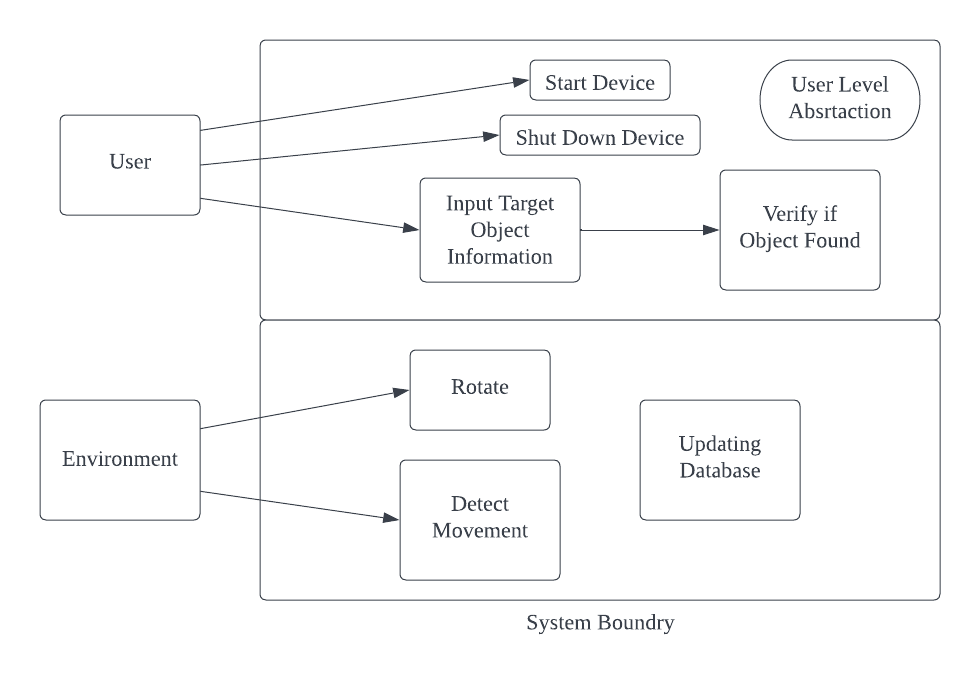
\includegraphics[scale=0.8]{Use.png}
    \caption{The Picture of Use Case Diagram}
\end{figure}
The Use Case Diagram shown above describes some actions that the user can interact with teh system. The line in the middle shows the boundaries between user and the internal program. The outmost large box shows the boundary for the whole system. All user can do is just to start and shut down the program. Th euser can also find the target object by typing the infromation about the object and verify if the object is found. The system will interact with the environment by rotating its camera and detecting the movement of the object in the room. It will also ba able to update its database when the position of the object is changed. 

\section{Functional Requirements}
The following are the functional requirements of the project. They are separated into 2 main parts: Image Processing and Storage, and UI Interface Menu.
\subsection{Image Processing and Storage Requirements}
\textbf{IPR1:} The device should be able to identify human's body.\\\\
\textbf{IPR2:} The device must be able to identify human's hand.\\\\
\textbf{IPR3:} The device must be able to take a photo automatically when required.\\\\
\textbf{IPR4:} The device should be able to identify all the small items being exposed to the camera.\\\\
\textbf{IPR5:} The device should be able to take a photo once the change of the location of an item is captured.\\\\
\textbf{IPR6:} The device should be able to differentiate one item from another items which are identified by the system through 3 main parameters,item\_shape, item\_color and item\_size.\\\\
\textbf{IPR7:} The device must be able to store all the photos into a file, and indicate the time when it was taken.\\\\
\textbf{IPR8:} The device must be able to name each item with a unique ID.\\\\
\textbf{IPR9:} The device should be able to arrange the photos stored in the file in ascending or descending order according to the time it was taken.\\\\
\textbf{IPR10:} The device should be able to arrange the photos stored in the file in ascending or descending order according to their IDs.
\subsection{UI Interface Menu Functional Requirements}
\textbf{UIR1:} The UI should be able to let user to choose whether to highlight a certain item or not.\\\\
\textbf{UIR2:} The UI should be able to let user to switch the ordering method.\\\\
\textbf{UIR3:} The UI must be able to notify the user when the WIFI signal is weak or unstable.\\\\
\textbf{UIR4:} The UI must be able to allow the user to view the system’s status at any given point in time

\section{Nonfunctional Requirements}
The next paragraphs will talk about about nonfunctional requirements in the designing of the smartVault, which will be discussed in several different parts. 
\subsection{Look and Feel Requirements}
\subsubsection{Appearance Requirements}
\textbf{APR1:} The device should not have exposed internal electronic wiring.\\\\
\textbf{APR2:} The sharp corners should not be exposed to the users annd shoudl be covered by some soft materials.
\subsubsection{style}
Not Applicable.
\subsection{Usability and Humanity Requirements}
\subsubsection{Easy of Use Requirements}
\textbf{EUR1:} The device should be easy to install in the roonm.\\\\
\textbf{EUR2:} Fonts, blanks and graphics shown on the screen should be big and visiable enough for the user to use without inserting wrong information.
\subsubsection{Personalization and Internationalization Requirements}
Not applicable.
\subsubsection{Learning Requirements}
\textbf{LR1:} The software part of the product should be easy to install.\\\\
\textbf{LR2:} The product should be easy to set up in its working environment.\\
\textbf{Rationale:} The device can identify objjects in teh room in a short tiime after powering up.
\subsubsection{Understandability and Politeness Requirements}
\textbf{UPR1:} The graphics used should be readeable and visiable to the user.\\
\textbf{Rationale:} Easy for clients to find objects the wish to find in the room.
\subsection{Accessibility Requirements}
\textbf{AR1:} The display window should be concise enough for user to understand
\subsection{Performance Requirements}
\subsubsection{Speed and Latency Requirements}
\textbf{SLR1:} The response time of the product to show the location of the object should be less than 5 seconds.
\subsubsection{Safety-Critical Requirements}
\textbf{SCR1:} The base of the device should be strong enough without falling from the floor.\\\\
\textbf{SCR2:} The device should not infringe on user's privacy.\\\\
\textbf{SCR3:} The rotating speed of the motor should be slow enough without hurting people.
\subsubsection{Precision and Accuracy Requirements}
\textbf{PAR1:} The time based value used in the device should be precised to minute.\\\\
\textbf{PAR2:} The location value used in the devce should be precised to whole number.\\\\
\textbf{PAR3:} Other numatic values used in the device should be rounded to one decimal place.
\subsubsection{Reliability and Avaliability Requirements}
\textbf{RAR1:} The device should not over-rotate to an unexpected angle.\\\\
\textbf{RAR2:} The device should be avaliable to work for the whole time of except for maintaince or updating time.
\subsubsection{Robustness or Fault-Tolerance Requirements}
\textbf{RFR1:} The data stored in the file should not be deleted or changed even after the program shuts down.\\\\
\textbf{RFR2:} The device should be able to notify user for an error occurs in the program.\\
\textbf{Rationale:} The user should be notified if he or she has a wrong input or havin inappropriate actions.
\subsubsection{Capacity Requirements}
\textbf{CR1:} The device sould be able to store the any information about the location of each object detected from the camera.
\subsubsection{Scalability or extensibility Requirements}
Not applicable.
\subsubsection{Longevity Requirements}
\textbf{LR1:} The device shoudl store the infromation about the objects until it is changed into a different environment.
\subsection{Operational and Environmental Requirements}
\subsubsection{Expected Physical Environment}
\textbf{EPE1:} The device is supposed to work in any indoor space.
\subsubsection{Requirements for Interfacing with Adjacent Systems}
Not applicable.
\subsubsection{Productization Requirements}
Not applicable.
\subsubsection{Release Requirements}
No applicable.
\subsection{Maintainability and Support Requirements}
\subsubsection{Maintenance Requirements}
\textbf{MR1:} The maintenance for the device should be done by the developers.
\subsubsection{Supportability Requirements}
\textbf{SR1:} The device is supported by any computers supports both C and python programming languages.
\subsubsection{Adaptability Requirements}
Not Applicable.
\subsection{Security Requirements}
\subsubsection{Access Requirements}
\textbf{AR1:} Any one except for the users is not allowed to access the any file that stores the information about the objects in the room.
\textbf{AR1:} Any one except for the users is not allowed to access the any file that stores the information about the objects in the room.
\subsubsection{Integrity Requirements}
\textbf{IR1:} Data in teh files should not be changed unnecessarily.\\\\
\textbf{IR2:} The files are locked whhen teh device shuts down.
\subsubsection{Privacy Requirements}
\textbf{PR1:} Other users are not allowed to access any file in the computer.\\
\textbf{PR2:} The camera should only work for a specific user.
\subsubsection{Audit Requirements}
Not applicable.
\subsubsection{Immunity Requirements}
Not applicable.
\subsection{Cultural and Political Requirements}
\subsubsection{Cultural Requirements}
Not applicable.
\subsubsection{Plitical Requirements}
Not applicable.
\subsection{Legal Requirements}
\subsubsection{Compliance Requirements}
\textbf{CR1:} The performance of the product should not violet the laws that protect the privacy of thee user.
\subsubsection{Standards Requirements}
Not applicable.

\section{Project Issues}

\subsection{Open Issues}

\subsection{Off-the-Shelf Solutions}

\subsection{New Problems}

\subsection{Tasks}

\subsection{Migration to the New Product}

\subsection{Risks}

\subsection{Costs}

\subsection{User Documentation and Training}

\subsection{Waiting Room}

\subsection{Ideas for Solutions}

\newpage

\bibliographystyle {plainnat}
\bibliography {../../refs/References}

\newpage

\section{Appendix}

This section has been added to the Volere template.  This is where you can place
additional information.

\subsection{Symbolic Parameters}

The definition of the requirements will likely call for SYMBOLIC\_CONSTANTS.
Their values are defined in this section for easy maintenance.

\subsection{Reflection}

The information in this section will be used to evaluate the team members on the
graduate attribute of Lifelong Learning.  Please answer the following questions:

\begin{enumerate}
  \item What knowledge and skills will the team collectively need to acquire to
  successfully complete this capstone project?  Examples of possible knowledge
  to acquire include domain specific knowledge from the domain of your
  application, or software engineering knowledge, mechatronics knowledge or
  computer science knowledge.  Skills may be related to technology, or writing,
  or presentation, or team management, etc.  You should look to identify at
  least one item for each team member.
  \item For each of the knowledge areas and skills identified in the previous
  question, what are at least two approaches to acquiring the knowledge or
  mastering the skill?  Of the identified approaches, which will each team
  member pursue, and why did they make this choice?
\end{enumerate}

\end{document}
